\title{Perculation}
\author{
        Andreas V. Solbr\aa \\
	      a.v.solbra@fys.uio.no \\
                University of Oslo\\
		 Department of Computational Physics
}

\documentclass[12pt]{article}
\usepackage{amsmath}
\usepackage{fullpage}
\usepackage{amsthm}
\usepackage{amsfonts}
\usepackage{graphicx}
\usepackage[english]{babel}
\usepackage[T1]{fontenc}
\usepackage{subfigure}
\usepackage{epstopdf}
\epstopdfsetup{update}
\usepackage[hyphens]{url}
\usepackage{gensymb}
\usepackage{verbatim}
%\usepackage{slashed}
\usepackage{amssymb}
\usepackage{amsfonts}
%\usepackage{caption}
%\usepackage{subcaption}
\newtheorem{thm}{Theorem}

%% Define a new 'leo' style for the package that will use a smaller font.
\makeatletter
\def\url@leostyle{%
  \@ifundefined{selectfont}{\def\UrlFont{\sf}}{\def\UrlFont{\small\ttfamily}}}
\makeatother
%% Now actually use the newly defined style.
\urlstyle{leo}


%\usepackage[utf8]{inputenc}
%\usepackage{textcomp}
%\usepackage[T1]{fontenc}




\newcommand{\Fig}[1]{Figure~\ref{#1}}
\newcommand{\fig}[1]{figure~\ref{#1}}
\newcommand{\eq}[1]{equation~\ref{#1}}
\newcommand{\Eq}[1]{Equation~\ref{#1}}

% Shortcuts for including equations
\newcommand{\beq}{\begin{equation}}
\newcommand{\eeq}{\end{equation}}
\def\ivec{\textbf{i}}
\def\jvec{\textbf{j}}
\def\kvec{\textbf{k}}
\def\uvec{\textbf{u}}
\def\vvec{\textbf{v}}
\def\xvec{\textbf{x}}
\def\rvec{\textbf{r}}
\def\Rvec{\textbf{R}}
\def\Fvec{\textbf{F}}
\def\S{\hat{S}}
\def\Svec{\hat{\textbf{S}}}
\def\H{\hat{H}}
\def\ro{\hat{\rho}}
\def\trace{\operatorname{Tr}}
\def\Lop{\hat{L}}
\def\etavec{\hat{\boldsymbol\eta}}
\def\X{\hat{X}}
\def\Y{\hat{Y}}
\def\etaop{\hat{\eta}}
\def\A{\hat{\textbf{A}}}
\def\B{\textbf{B}}
\def\aop{\hat{a}}
\def\aopd{\hat{a}^\dagger}
\def\bop{\hat{b}}
\def\bopd{\hat{b}^\dagger}




% Document formatting
\setlength{\parindent}{0mm}
\setlength{\parskip}{1.5mm}

% Hyper refs
\usepackage[pdftex,colorlinks,breaklinks]{hyperref}
\usepackage{listings}
\usepackage{color}
\usepackage{textcomp}
\definecolor{listinggray}{gray}{0.9}
\definecolor{lbcolor}{rgb}{0.9,0.9,0.9}
\definecolor{pink}{RGB}{255, 119, 255}
\lstset{
	backgroundcolor=\color{lbcolor},
	tabsize=4,
	rulecolor=,
	language=c++,
        basicstyle=\scriptsize,
        upquote=true,
        aboveskip={1.5\baselineskip},
        columns=fixed,
        showstringspaces=false,
        extendedchars=true,
        breaklines=true,
        prebreak = \raisebox{0ex}[0ex][0ex]{\ensuremath{\hookleftarrow}},
        frame=single,
        showtabs=false,
        showspaces=false,
        showstringspaces=false,
        identifierstyle=\ttfamily,
        keywordstyle=\color[rgb]{0,0,1},
        commentstyle=\color[rgb]{0.133,0.545,0.133},
        stringstyle=\color[rgb]{0.627,0.126,0.941},
	title=\lstname
}

\newcounter{subproject}
\renewcommand{\thesubproject}{\alph{subproject}}
\newenvironment{subproj}{
\begin{description}
\item[\refstepcounter{subproject}(\thesubproject)]
}{\end{description}}
\date{\today}

\begin{document}
 \maketitle
 \begin{abstract}
The goal of this project is to get used to some of the concepts in percolation.
 \end{abstract}
\section{Generating percolation clusters}
We begin by using Matlab to generate and visualize percolation clusters. We generate an $N\times N$ matrix of random uniform numbers then set each element equal to 1 if it is larger than some chosen $\epsilon$, and 0 if it is smaller. The we can then color the different connecting 1s in different colors, in order to study the formation of clusters. Some examples of this is shown in figure \ref{fig:1}.

\begin{figure}[ht]
\centering
\subfigure[$\epsilon = 0.4$]{
	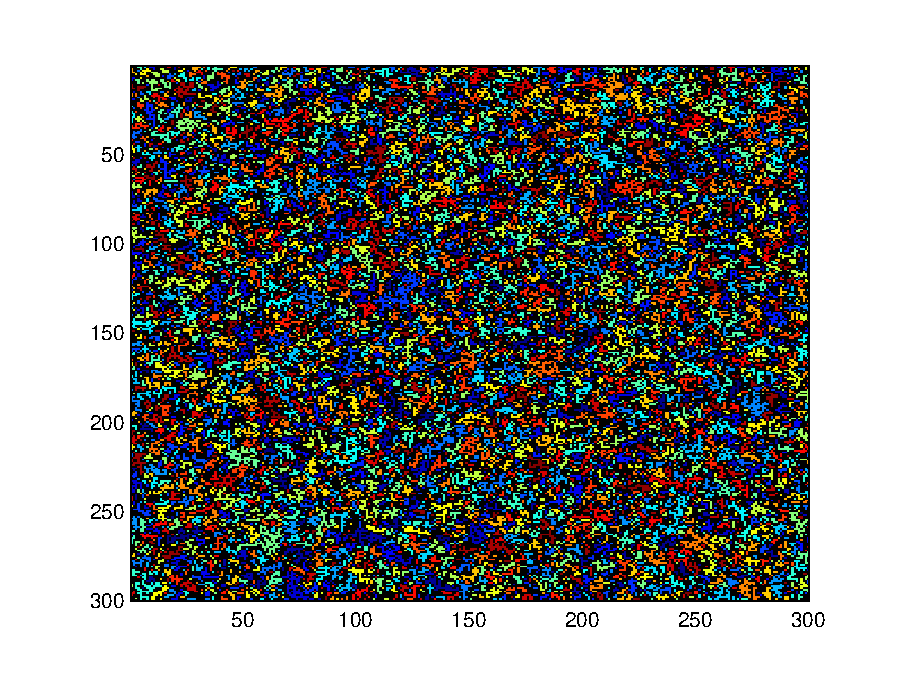
\includegraphics[width=7cm]{eps4.eps}
	\label{fig:subfig11}
}
\subfigure[$\epsilon = 0.5$]{
	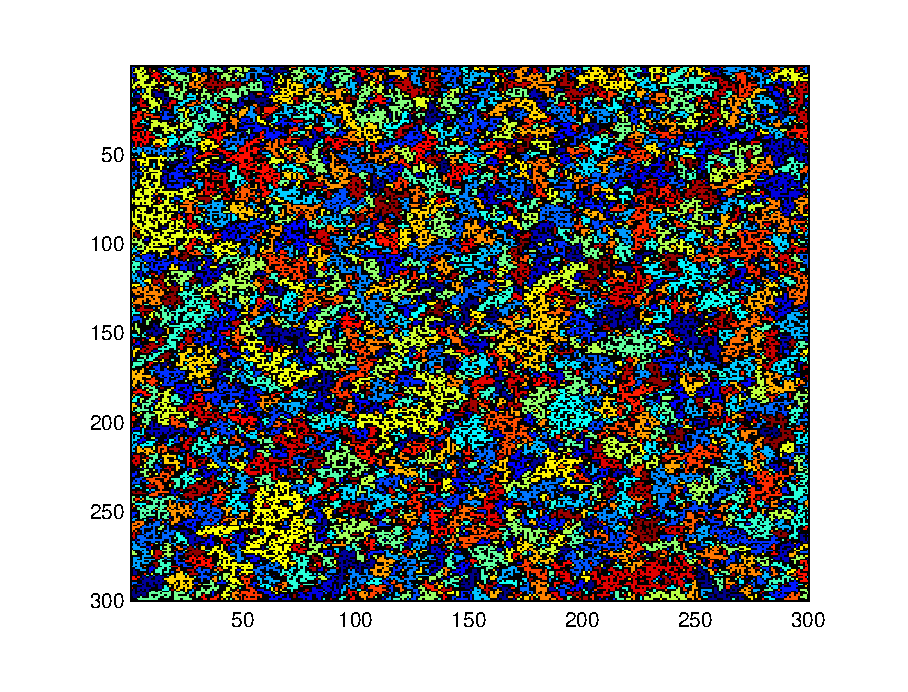
\includegraphics[width=7cm]{eps5.eps}
	\label{fig:subfig12}
}
\subfigure[$\epsilon = 0.6$]{
	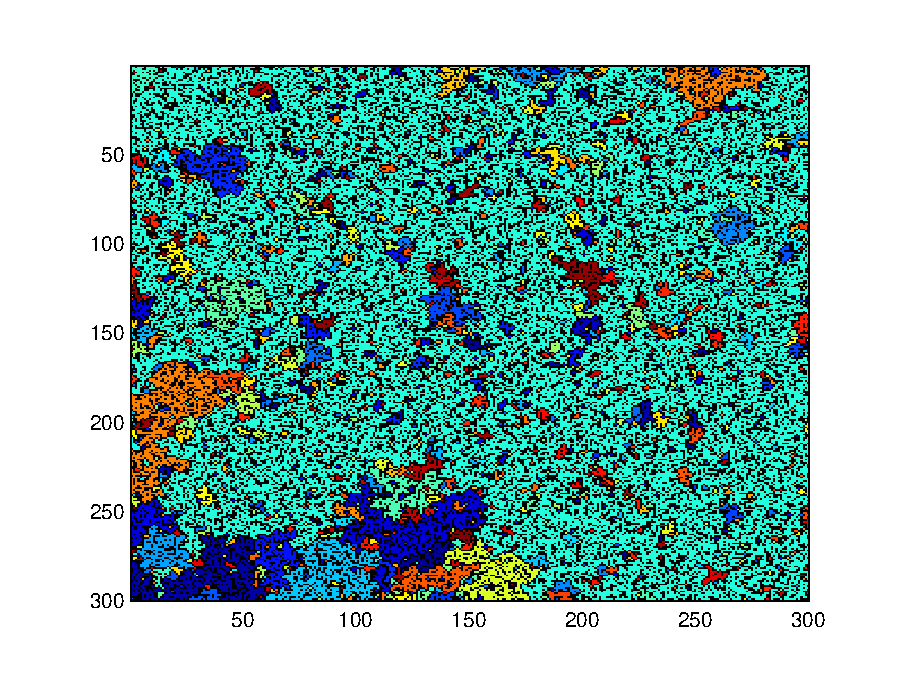
\includegraphics[width=7cm]{eps6.eps}
	\label{fig:subfig13}
}
\subfigure[$\epsilon = 0.7$]{
	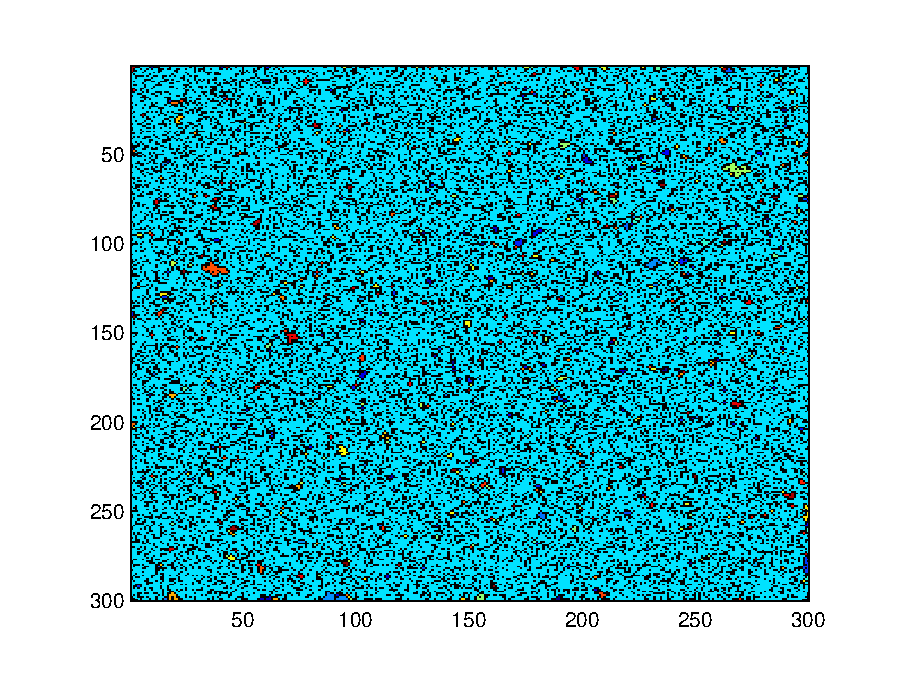
\includegraphics[width=7cm]{eps7.eps}
	\label{fig:subfig14}
}
\caption[Optional caption for list of figures]{The plots show cluster formation for different values of $\epsilon$.}
\label{fig:1}
\end{figure}

For infinitely large grids, there is a critical quantity called the percolation threshold, $p_c$, so that if the probabilty $p$ of a site beeing occupied is larger than $p_c$, there is a so-called {\it spanning} or {\it percolation cluster} which goes infinitely far in any direction. An interesting quantity is then the probability that a site is a part of such a spanning cluster. We call this $P(p)$. We cannot measure this on a computer, we can, however, measure its finite counterpart, $P(p,L)$. $P(p)$ has the form $P(p) = (p-p_c)^\beta$, where in this case $p_c = 0.59275$. We can assume that $P(p,L)$ takes the same form, and try to measure $\beta$ for the finite versions. The results of some such atempts are shown in figure \ref{fig:2}. We see that there is there are some differences between the finite and infinite case. For instance, in the infinite case $P(p)$ is zeros below $p_c$. In the finite case there is always a non-zero probability that a connecting cluster exists, so the curve is spread out a bit. 
We also see that the value for $\beta$ we measure is dependent on the system size. The value for $\beta$ for different values of $L$ is shown in figure \ref{fig:beta}. The limit of $\beta$ for $L\rightarrow \infty $ has been shown to be around 0.13.

\begin{figure}[ht]
\centering
\subfigure[$L=100$]{
	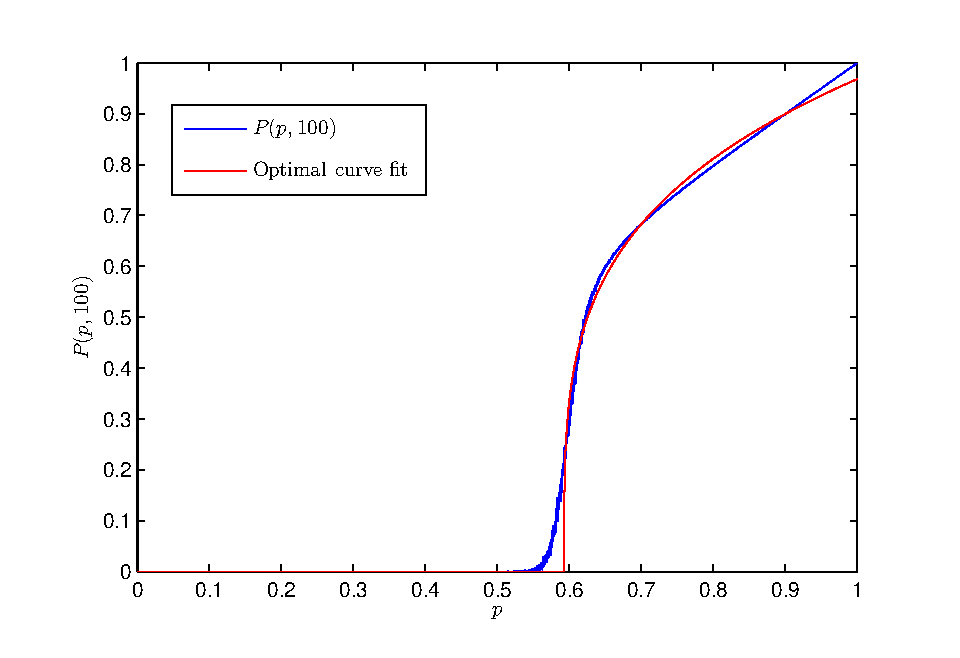
\includegraphics[width=7cm]{betaFit100.eps}
	\label{fig:subfig21}
}
\subfigure[$L=1000$]{
	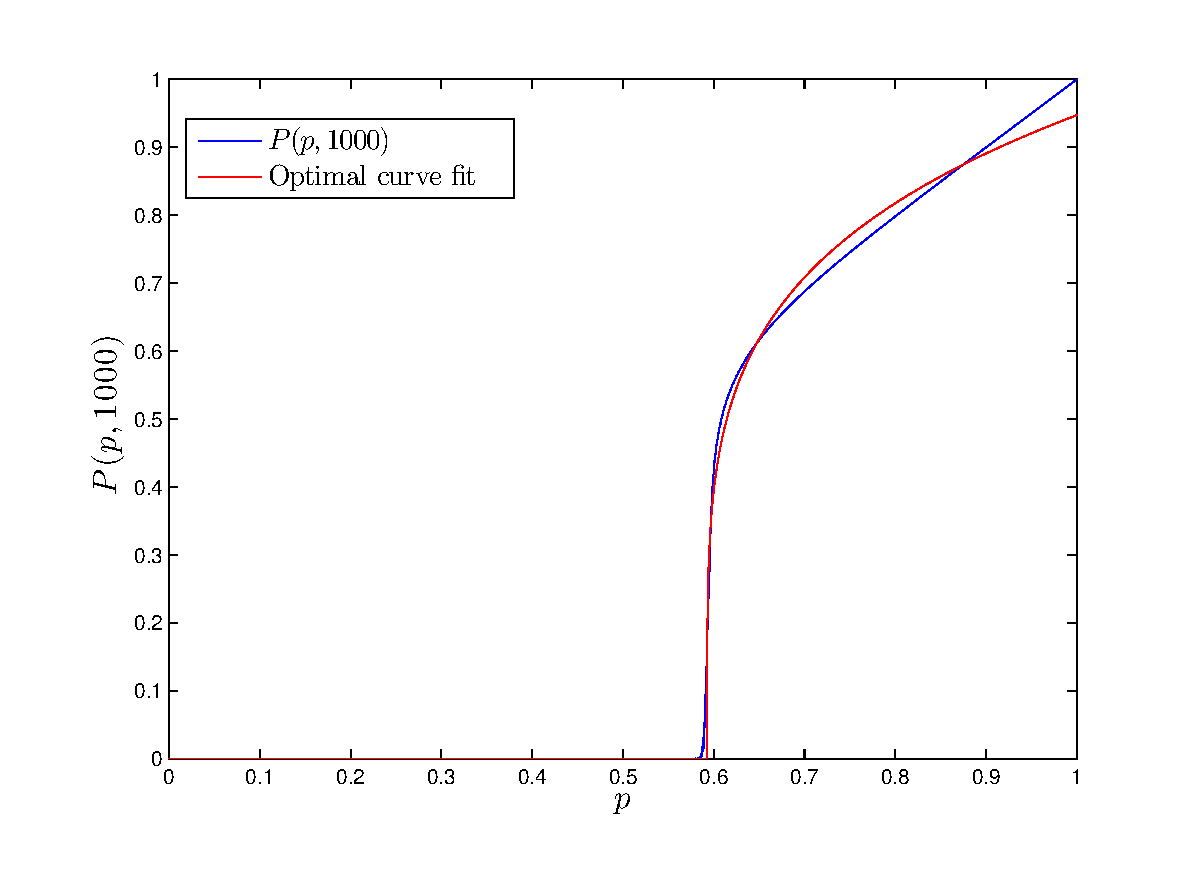
\includegraphics[width=7cm]{betaFit1000.eps}
	\label{fig:subfig22}
}
\caption[Optional caption for list of figures]{The plots show the best fit of the data to the theoretical curve $P(p) = (p-p_c)^\beta$}
\label{fig:2}

\end{figure}

\begin{figure}[ht]
\centering

	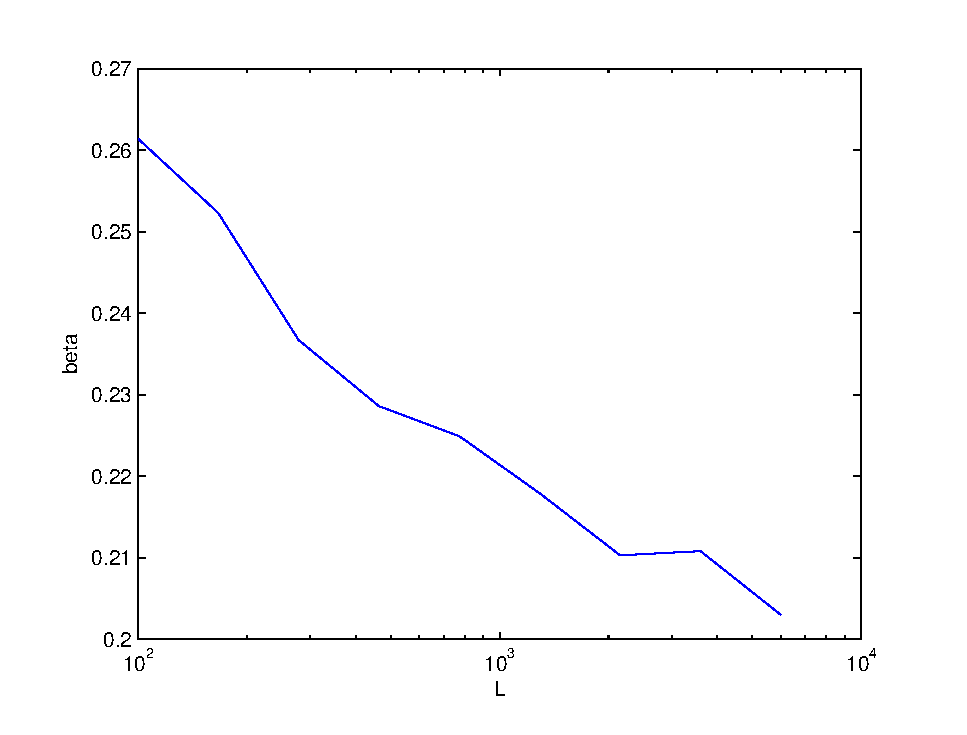
\includegraphics[width=13cm]{differentbetas.eps}
	%\label{fig:subfig51}


\caption[Optional caption for list of figures]{The figure shows the optimal values of $\beta$ for various $L$.}
\label{fig:beta}
\end{figure}
 

\section{Determining the exponent of power-law distributions}
We generate the following set of data points in Matlab: 
\begin{verbatim}
 z = rand(1e6,1).^(-3+1);
\end{verbatim}
What is the probability distribution for this set of points? A straight forward approach is to simply make a normalized histogram of the data set. This will be a good approximation for a big data set. However, since a lot of the large values are very unlikely, we can make a better histogram if we use a logarithmic bin size. This will give a somewhat better view of the statistics. 

A more sophisticated approach would be to find the cumulative distribution, $P(Z>z)$, and the find the probability density as 
\begin{equation}
 f_Z(z) = {dP(Z>z) \over dz}
\end{equation}
We can find $F_Z(z)$ by using a numerical derivative. However we risk running into some problems using this method if a bin does not contain any new points. We assume that $f(u) \propto u^\alpha$, and we want to measure $\alpha$. If we try to do linear regression on the logarithms, we end up with $log(0)$ for one or more values. Another, more stable approach is to note that with $f(u) \propto u^\alpha$, then $F(u) = 1-u^{\alpha+1}$. We can then measure $\alpha+1$ from a log-log plot of $1-F(u) = z^{\alpha+1}$. The results of these different approaches are shown in figre \ref{fig:4}, and we can measure $\alpha \approx 3/2$. We should note that using the latter method will allow us to use a much finer grid spacing, which is needed to get close to the correct value.

\begin{figure}[ht]
\centering
\subfigure[Probability density]{
	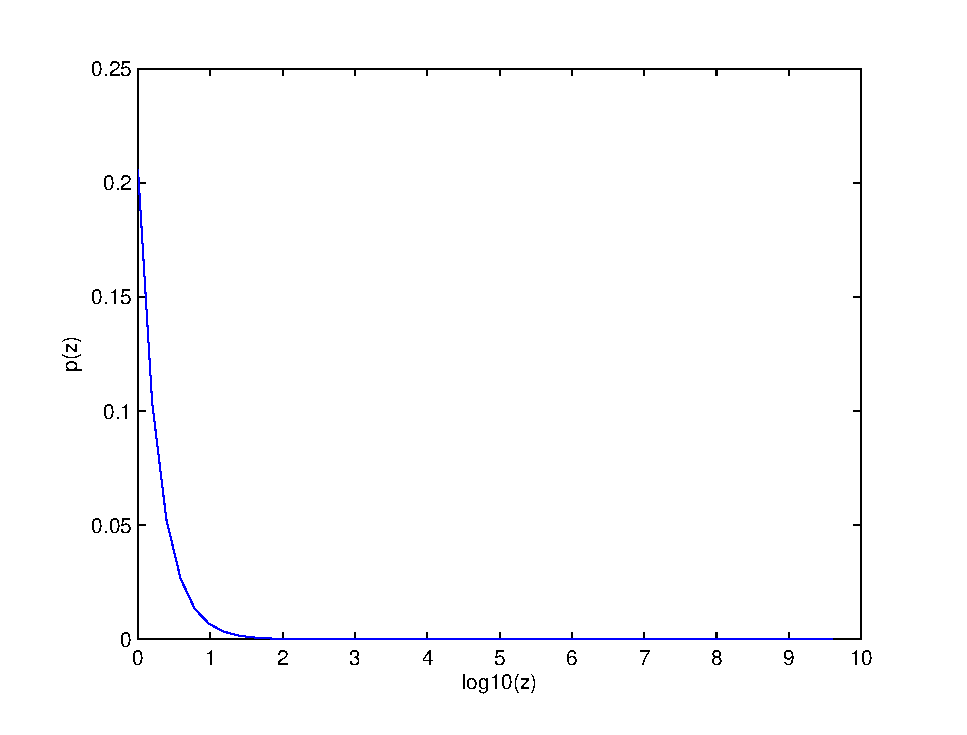
\includegraphics[width=7cm]{pdf.eps}
	\label{fig:subfig41}
}
\subfigure[log-log of probability density]{
	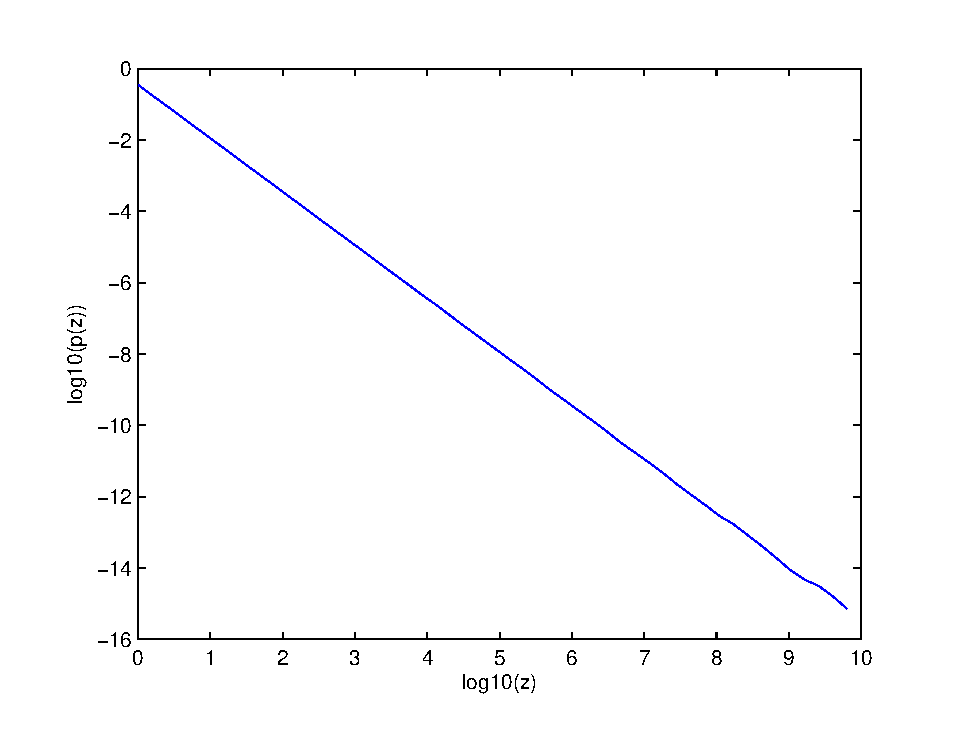
\includegraphics[width=7cm]{loglog_pdf.eps}
	\label{fig:subfig42}
}
\subfigure[cumulative probability]{
	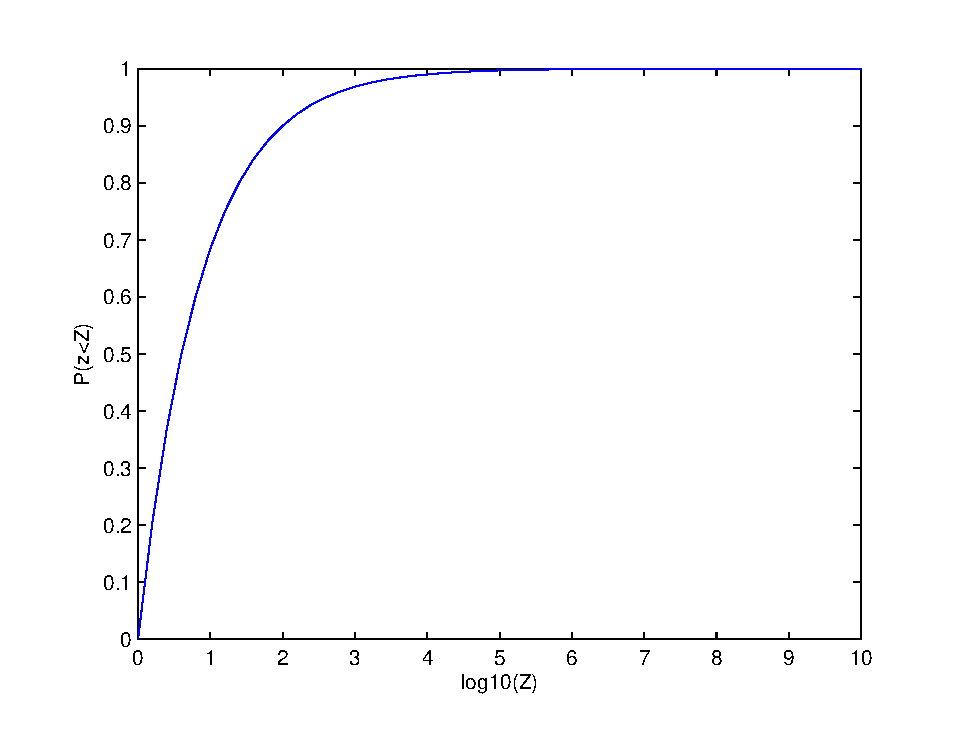
\includegraphics[width=7cm]{cumul.eps}
	\label{fig:subfig43}
}
\subfigure[log-log of cumulative probability]{
	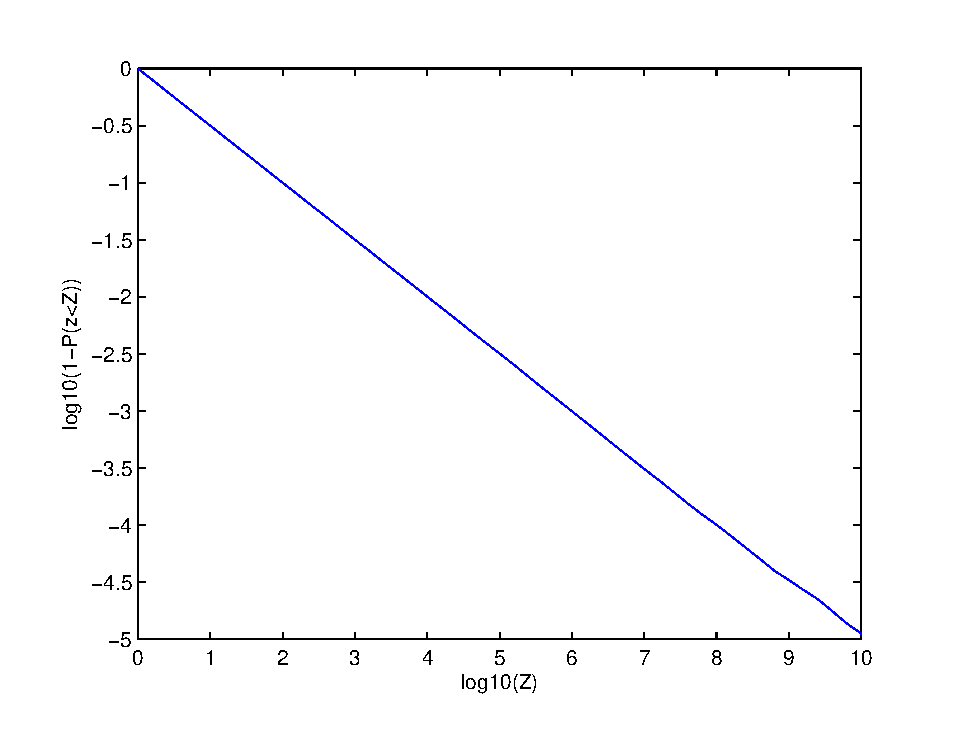
\includegraphics[width=7cm]{loglog_cumul.eps}
	\label{fig:subfig44}
}
\caption[Optional caption for list of figures]{The plots show the best fit of the data to the theoretical curve $P(p) = (p-p_c)^\beta$}
\label{fig:4}
\end{figure}

\section{Cluster number density $n(s,p)$}
The cluster number density is the probability for a random cluster to be of a particular size. It is espescially interesting to investigate this for $p$ close to $p_c$. Figure \ref{fig:5} shows $n(s,p)$ for p above and below $p_c$. 


\begin{figure}[ht]
\centering
\subfigure[$p>p_c$]{
	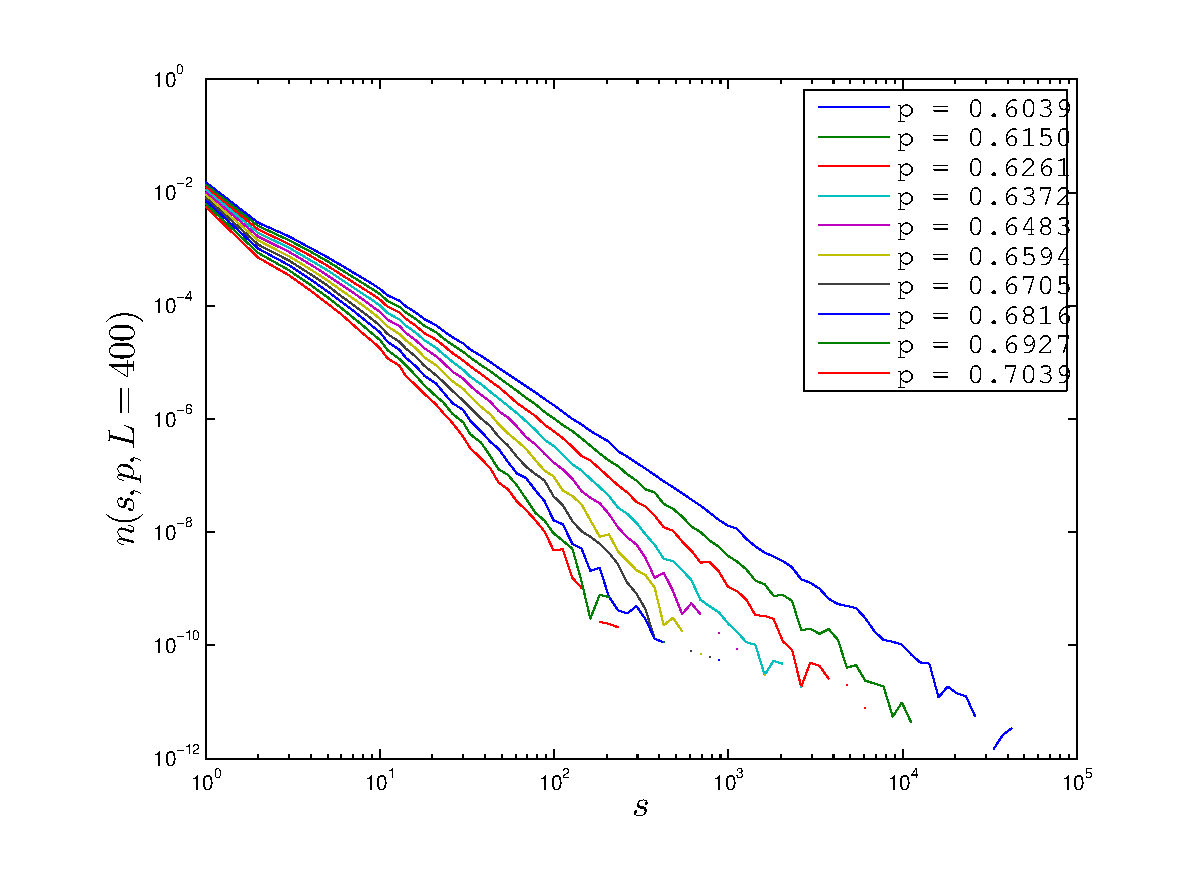
\includegraphics[width=7cm]{pabove.eps}
	\label{fig:subfig51}
}
\subfigure[$p<p_c$]{
	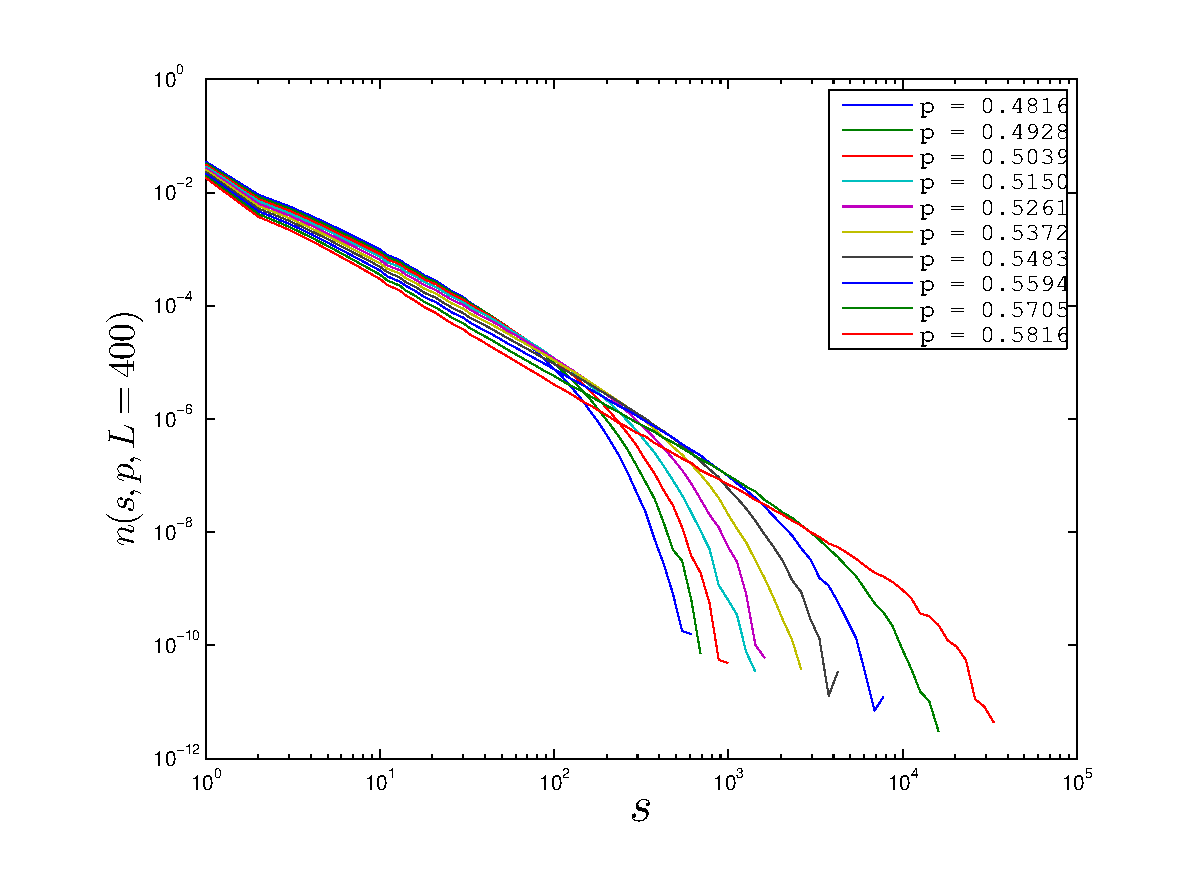
\includegraphics[width=7cm]{pbelow.eps}
	\label{fig:subfig52}
}
\caption[Optional caption for list of figures]{The plots show $n(s,p,L=400)$ for various $p$.}
\label{fig:5}
\end{figure}

We can use this data to estimate the scaling of $s_\xi \propto |p-p_c|^{-1/\sigma}$. $s_\xi$ is a typical cut-off length of the cluster size, and we can take as the definition the value where $n(s,p)/n(s,p_c) = F(s/s_\xi) = 0.5F_\text{max}$, i.e. whereever the ratio of the densities have fallen to half its maximal value. Figure \ref{fig:sigma} shows these half points geometrically, as well as the the experimental values of the cut-off lengths, compared to the theoretical result for an optimal value of $\sigma$. 


\begin{figure}[ht]
\centering
\subfigure[investigations of $s_\xi$]{
	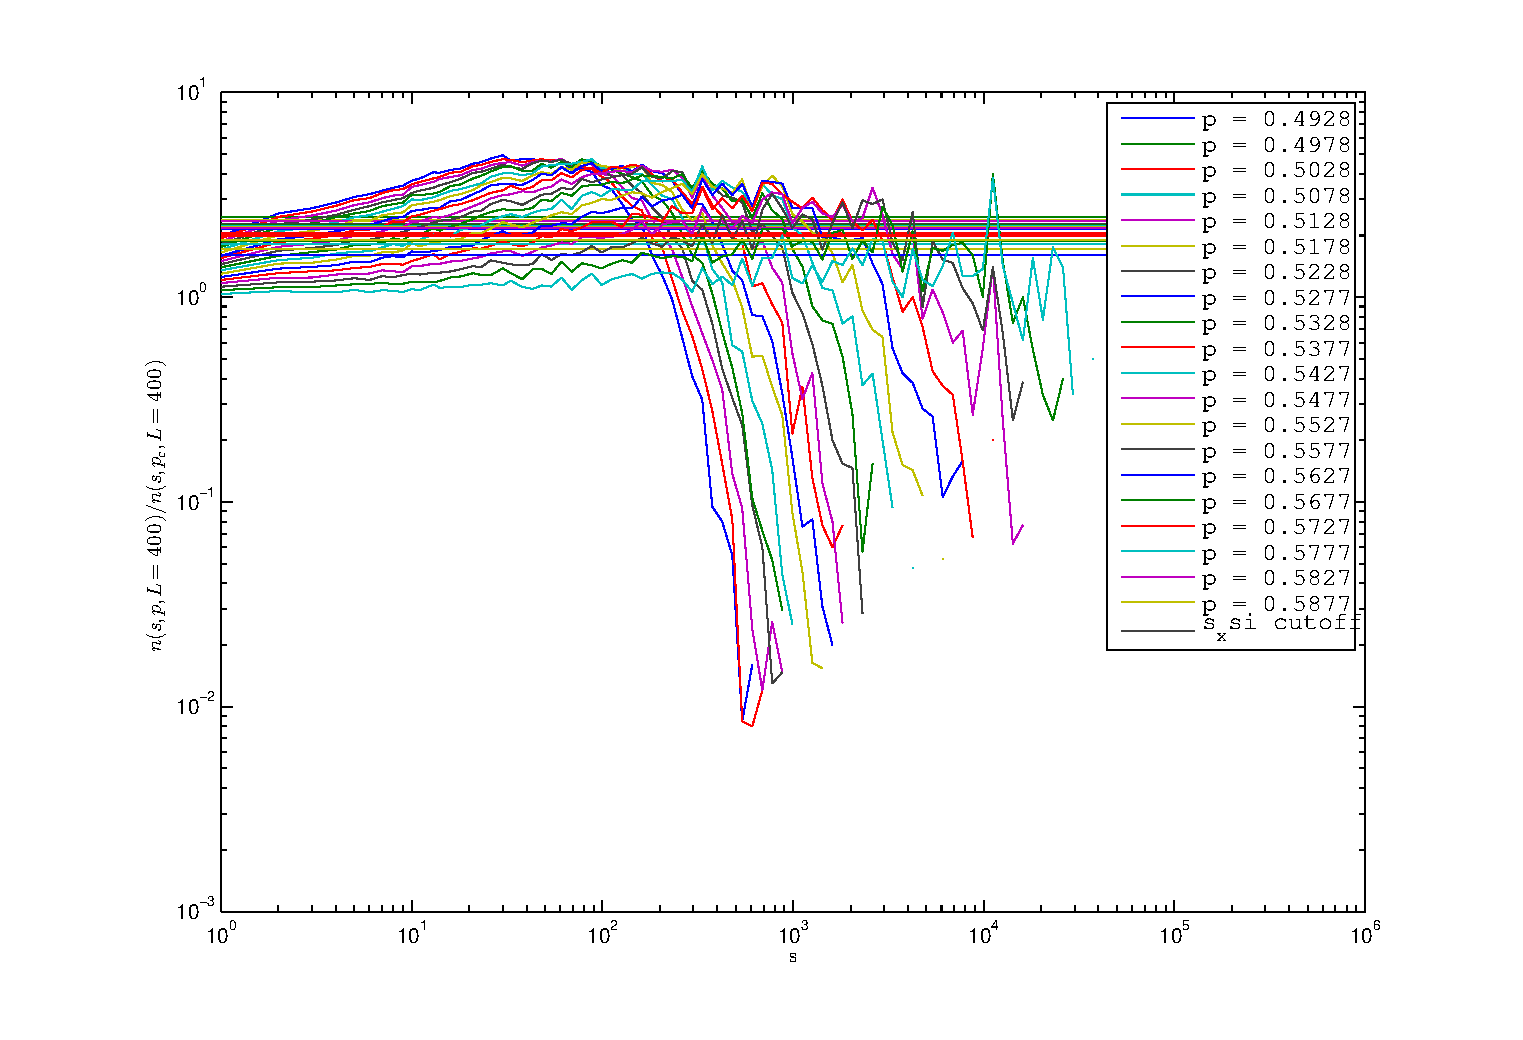
\includegraphics[width=7cm]{relativeexample.eps}
	\label{fig:subfigs1}
}
\subfigure[scaling of $s_\xi$]{
	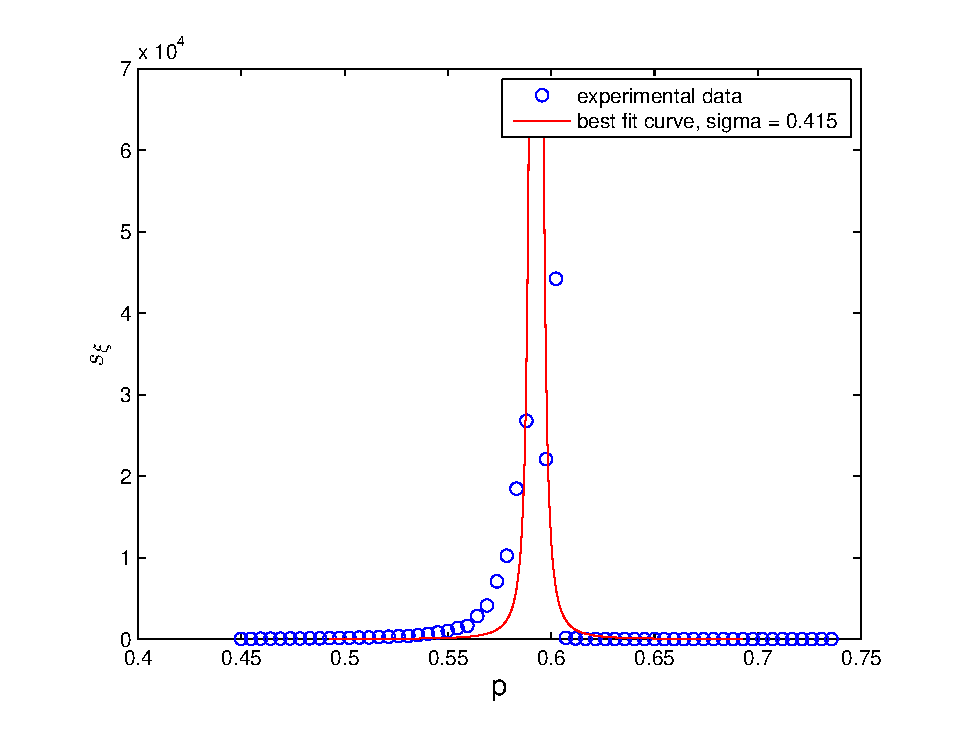
\includegraphics[width=7cm]{sigmaplot.eps}
	\label{fig:subfigs2}
}
\caption[Optional caption for list of figures]{The plots illustrate the method for approximating $s_\xi$ for various $p$, as well as the results compared to the theoretical curve $|p-p_c|^{-1/\sigma}$}
\label{fig:sigma}
\end{figure}


We can also estimate $n(s,p_c,L)$ for different values of $L$, as shown in figure \ref{fig:6}. From theoretical considerations, we have $n(s,p_c) = Cs^{-\tau}$, where in the infinite case $\tau = 187/91 \approx 2.05$. We can measure $\tau$ for our finite cases. We strip off the end points that are heavily effected by the finite size of the system. and measure the increase of the loglog-plot. For $L=512$, we find $\tau = 1.89$.
\begin{figure}[ht]
\centering

	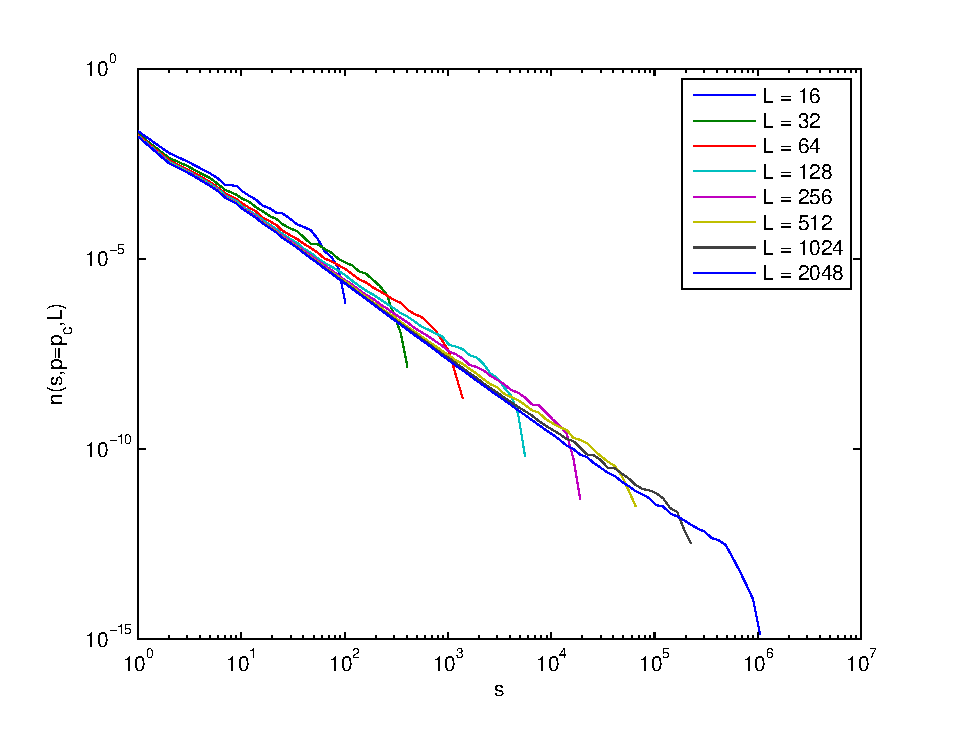
\includegraphics[width=13cm]{differentLs.eps}
	%\label{fig:subfig51}


\caption[Optional caption for list of figures]{The plots show $n(s,p=p_c,L)$ for various $L$.}
\label{fig:6}
\end{figure}



\section{Mass scaling of percolating cluster}
We can also investigate the average mass of the percolating cluster at $p=p_c$ for various system sizes. We should note that there is no guarantee that there is a percolating cluster for our finite size systems, and trials where none is found should be discarded. Figure \ref{fig:7} shows the distribution of a sample run, as well as a log-log plot of the masses and system sizes. We find that 
\begin{equation}
 M(L) \propto L^{D},
\end{equation}
where $D \approx 1.88$.



\begin{figure}[ht]
\subfigure[a typical mass distribution]{
	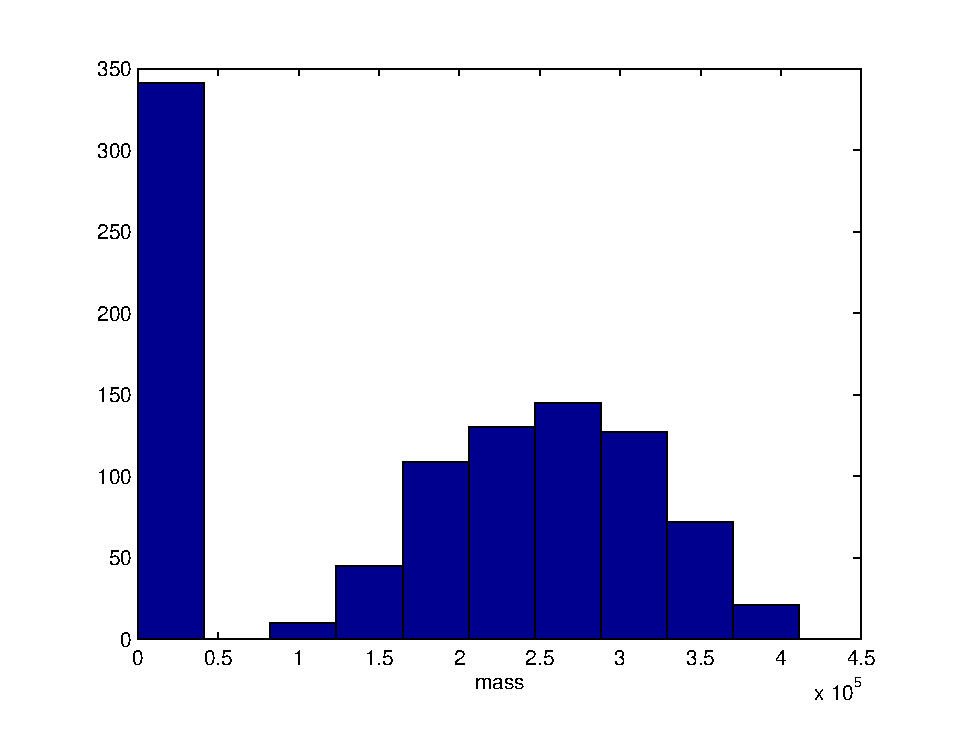
\includegraphics[width=7cm]{masshistexample.eps}
	\label{fig:subfig71}
}
\subfigure[loglog of average means]{
	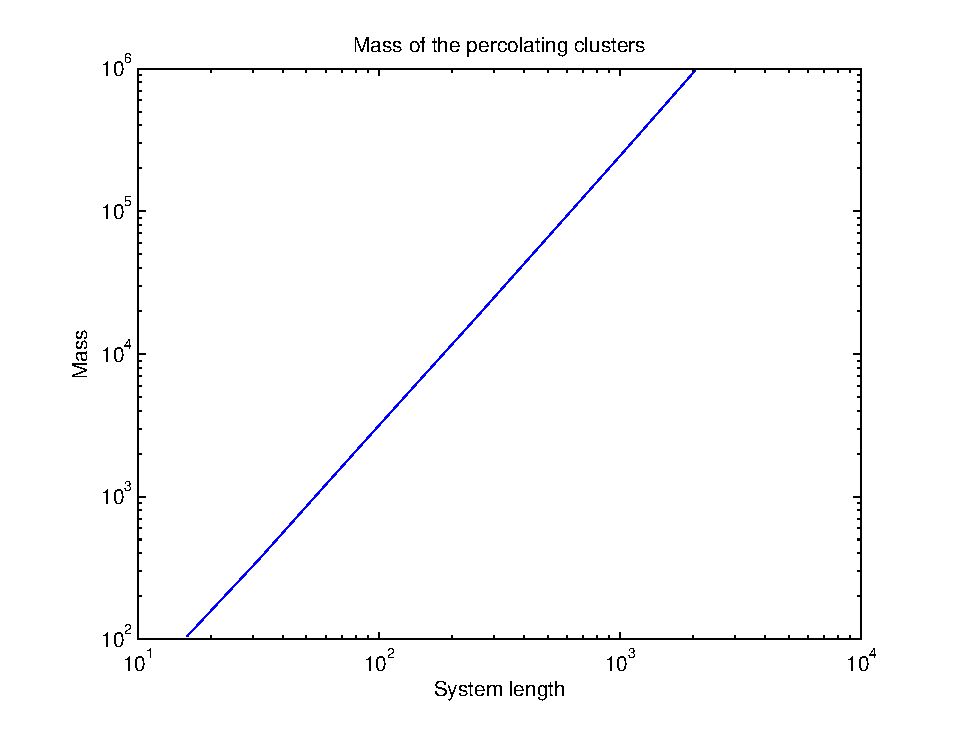
\includegraphics[width=7cm]{mass.eps}
	\label{fig:subfig72}
}

\caption[Optional caption for list of figures]{The figure shows the average mass of the percolating clusters for various system sizes, as well a a typical mass distribution.}
\label{fig:7}
\end{figure}

\clearpage
\section{Finite Size Scaling}
In this exercise we will use a finite size scaling ansatz to provide estimates of $\nu$, $p_c$, and the average percolation probability $\langle p \rangle$ in a system of size $L$.

We define $p_{\Pi=x}$ so that
\begin{equation}
 \Pi(p_{\Pi=x}) = x,
\end{equation}
notice that $p_{\Pi=x}$ is a function of system size $L$ used for the simulation. We can investigate the form of this function by finding $\Pi$ for several system sizes. The result of this is shown in figure \ref{fig:8}. The results indicate that $|p_{\Pi=x} - p_c| = C_xL^{-1/\nu}$, where the exponent is independent of $x$. 


\begin{figure}[ht]
\subfigure[$x=0.3$]{
	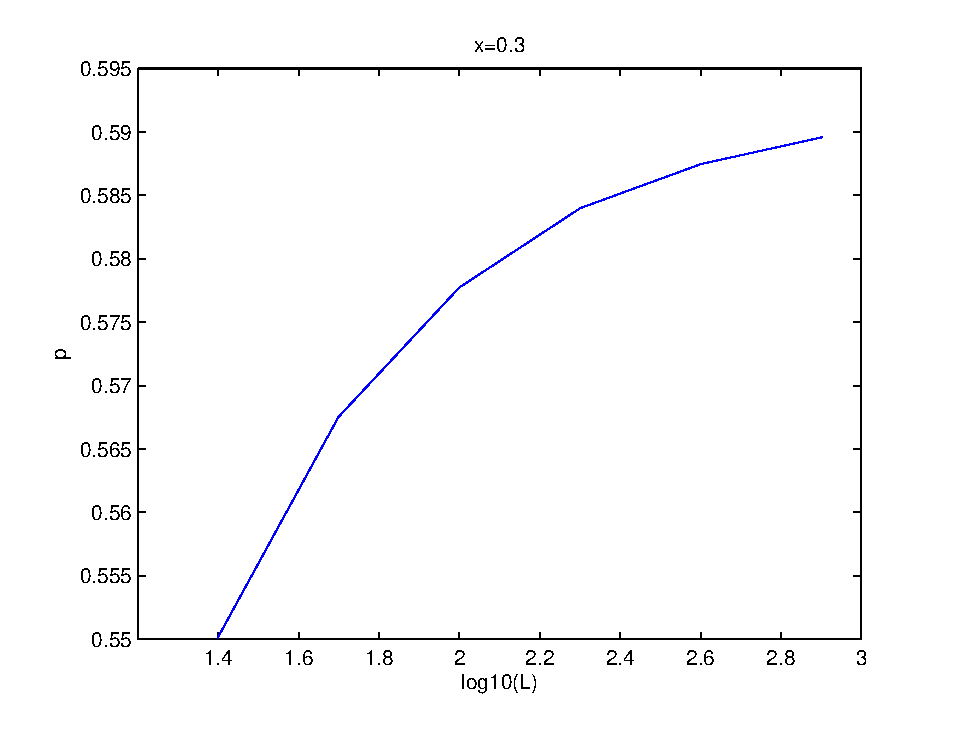
\includegraphics[width=7cm]{fss3.eps}
	\label{fig:subfig81}
}
\subfigure[$x=0.3$]{
	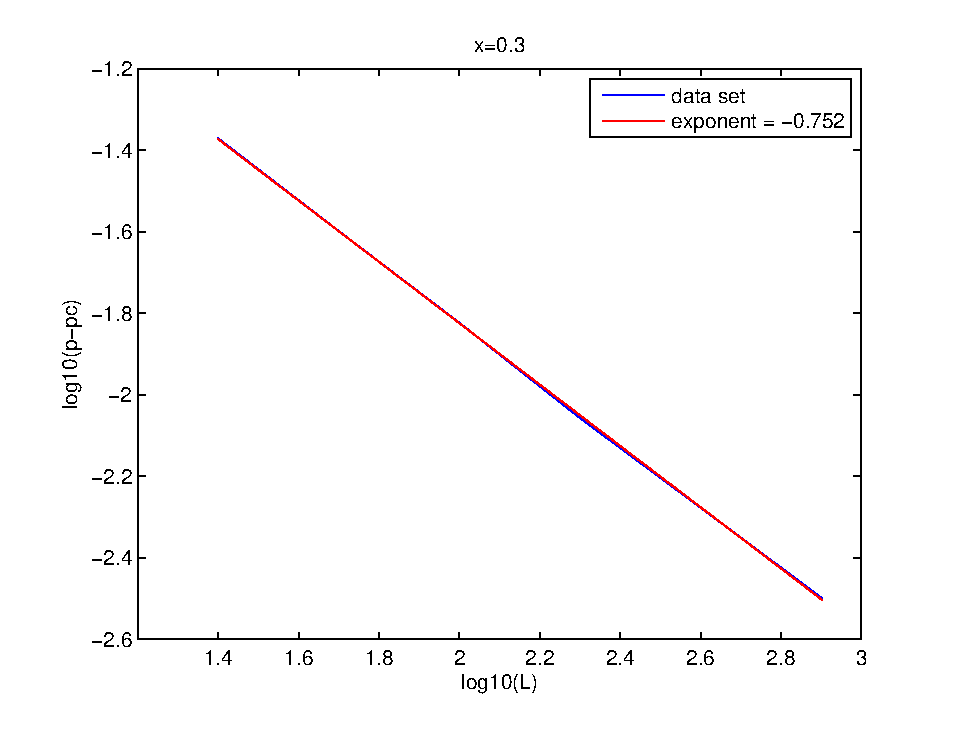
\includegraphics[width=7cm]{fssloglog3.eps}
	\label{fig:subfig82}
}
\subfigure[$x=0.8$]{
	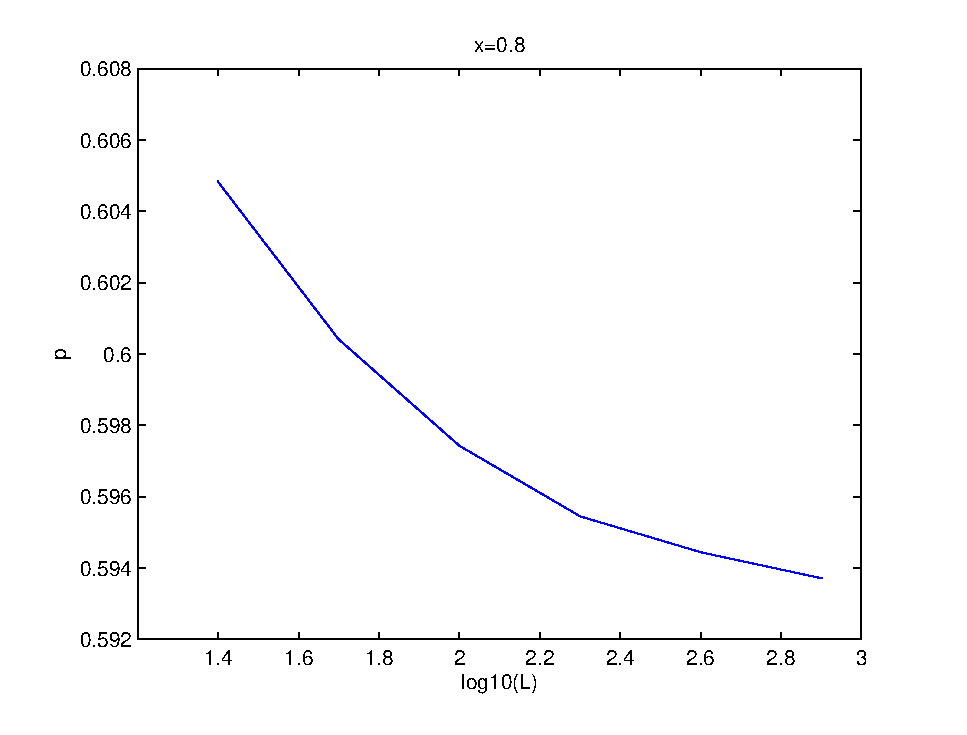
\includegraphics[width=7cm]{fss8.eps}
	\label{fig:subfig83}
}
\subfigure[$x=0.8$]{
	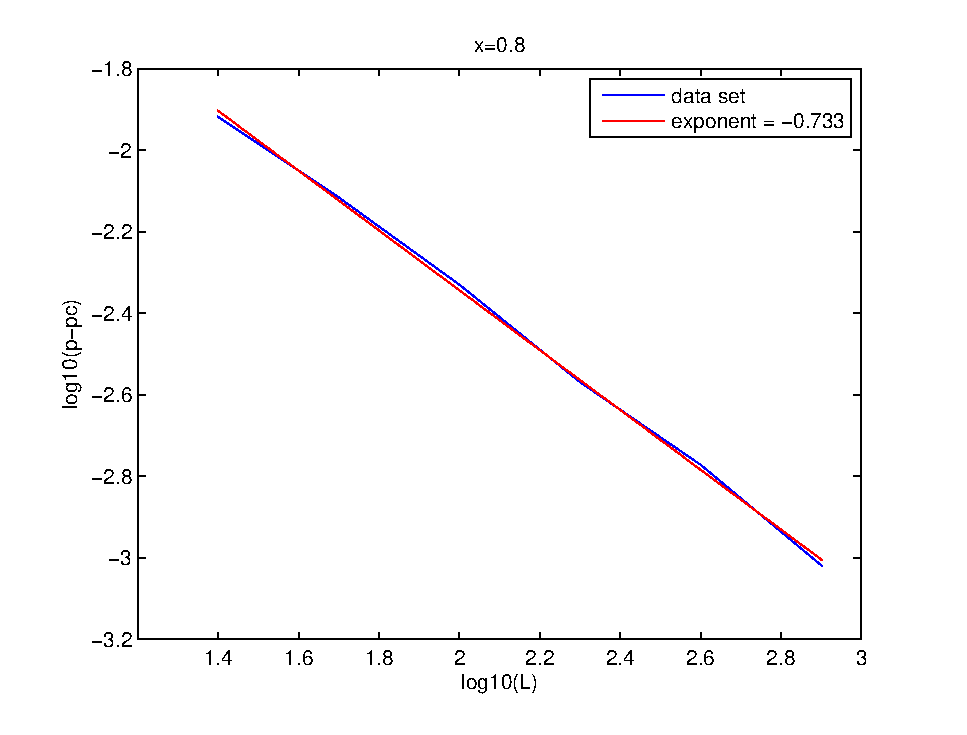
\includegraphics[width=7cm]{fssloglog8.eps}
	\label{fig:subfig84}
}
\caption[Optional caption for list of figures]{The figures show $p_{\Pi=x}$ as a function of $L$.}
\label{fig:8}
\end{figure}

According to scaling theory we have $p_{x_1} - p_{x_2} = (C_{x_1} - C_{x_2})L^{-1/\nu}$ We can measure the exponent as $\nu$ by plotting $\log(p_{\Pi=0.8}-p_{\Pi=0.3})$ as a function of $\log(L)$. Such a procedure give the result $\nu = 1.32$, which is very close to the theoretical value of $\nu = 4/3$.

We can also approximate $p_c$ as scaling theory predicts that 
\begin{equation}
 p_{\Pi = x} = p_c + C_x L^{-1/\nu}
\end{equation}
and so we can plot $p_{\Pi = x}$ as a function of $L^{-1/\nu}$, and find $p_c$ as the intersection of the of the plots with the y-axis. This is shown in figure \ref{fig:9}, and we find $p_c$ as $p_c = 0.5929$, which can be compared to the best known value $p_c = 0.59275$.

\begin{figure}[ht]
\centering

	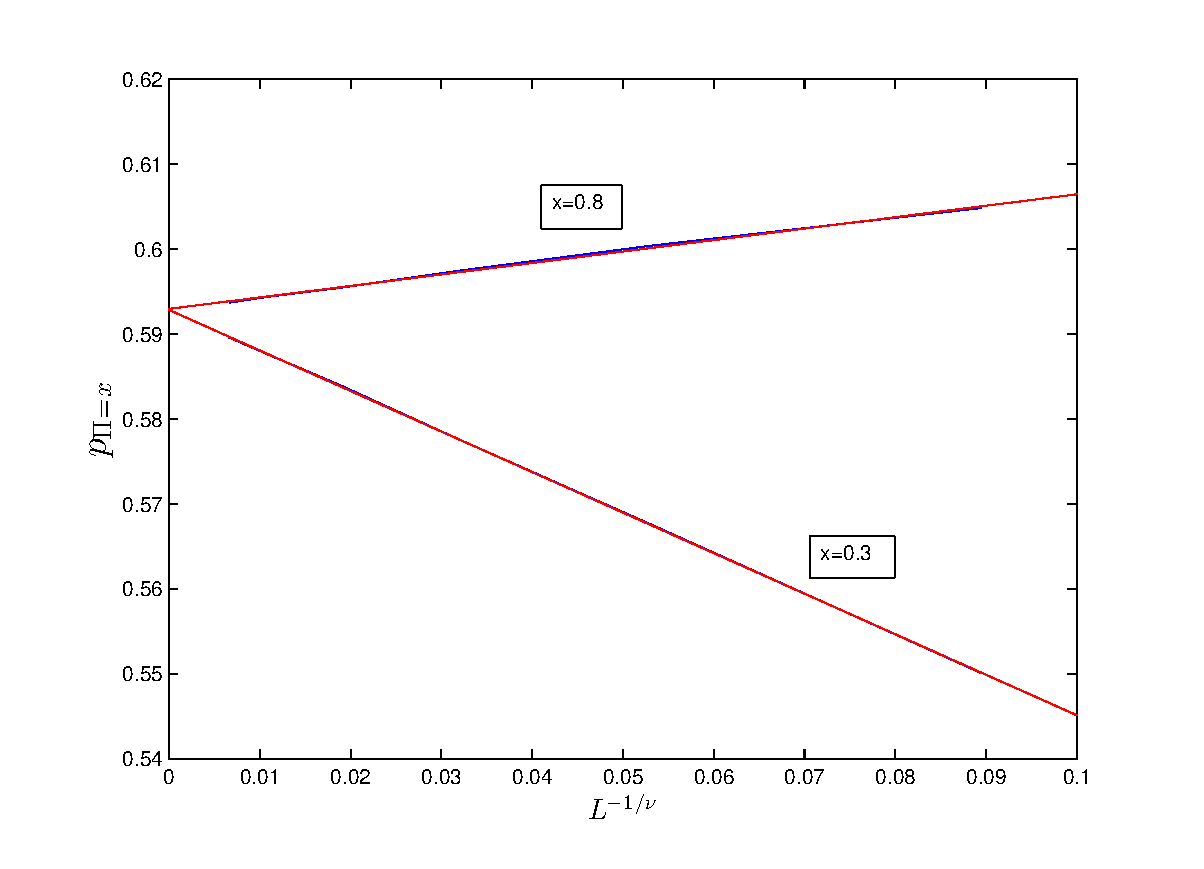
\includegraphics[width=13cm]{intersection.eps}
	%\label{fig:subfig51}


\caption[Optional caption for list of figures]{The plots show the $p_{\Pi = x} = p_c + C_x L^{-1/\nu}$ for various $x$.}
\label{fig:9}
\end{figure}

We can also make a data collapse plot for $\Pi(p,L)$ to find the shape of $\Phi(x)$. This is shown in figure \ref{fig:dcp}

\begin{figure}[ht]
\centering

	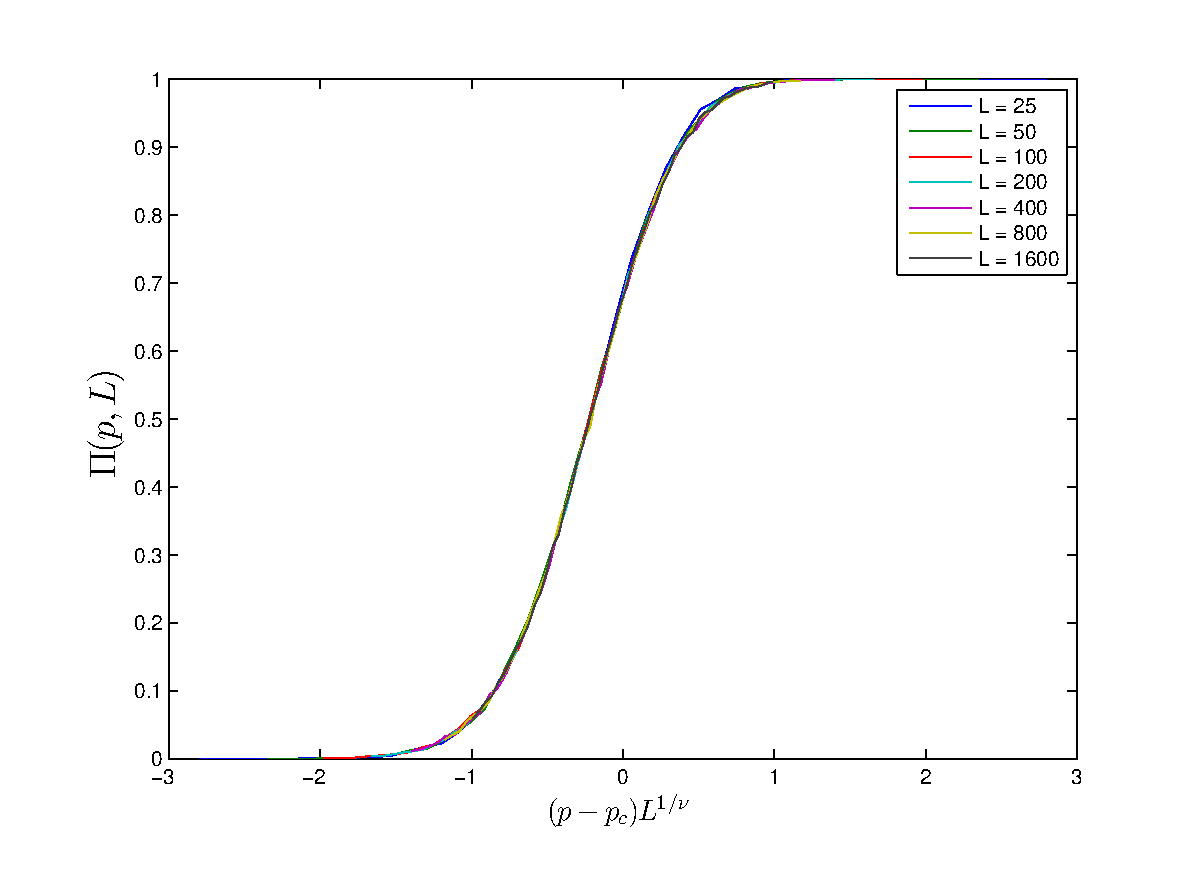
\includegraphics[width=13cm]{datacollpi.eps}
	%\label{fig:subfig51}


\caption[Optional caption for list of figures]{The figure shows a data collapse plot of $\Pi(p,L)$.}
\label{fig:dcp}
\end{figure}

\section{Singly connected bonds}
Singly connected bonds are sites in a percolating cluster that are sites that are essential for the percolation. If we imagine the percolating cluster as area where a liquid can flow through a media, all the liquid will flow through the singly connected bonds. 

\subsection{Locating singly connected bonds} \label{sec:lscb}
One way to find the singly connected bonds is to start in one end of the cluster and let to walkers traverse it. One by always clinging to the left side of the cluster wall, and one by always clinging to the right side. If both of the walkers go through a cell, then that cell must be a singly connected bond. One way to understand why this method works is that all other paths through the cluster must lie between the rightmost path and the leftmost path. So if they coincide at any site, so must all the other paths. An example of an application of this algoright is shown in figure \ref{fig:10}. Note that some of the bonds have different colors because the walker might pass through the site several times.

\begin{figure}[ht]
\centering

	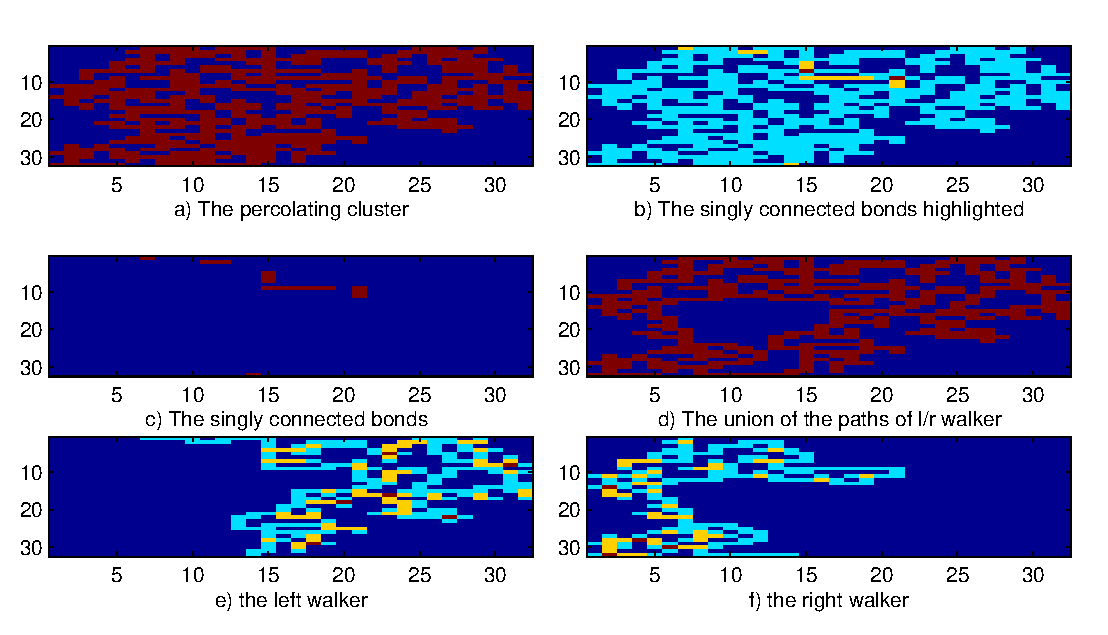
\includegraphics[width=13cm]{singlyconnected.eps}
	%\label{fig:subfig51}


\caption[Optional caption for list of figures]{The plot shows properties of a percolating cluster found by the algorithm  described in section \ref{sec:lscb}}
\label{fig:10}
\end{figure}

We are interested in finding the mass of the singly connected bonds as a function of $L$. A simulation using 10000 experiments for $L\in\{ 32,64,128,256,512,1024, 2048 \}$. The results are shown in figure \ref{fig:11}, and we find that $M_{SC} \propto L^{D_{SC}}$, where $D_{SC} \approx 0.76$. This is in good agreement with the theoretical value of $D_{SC} = 1/\nu = 3/4$. We will not show this expression here. 

\begin{figure}[ht]
\centering

	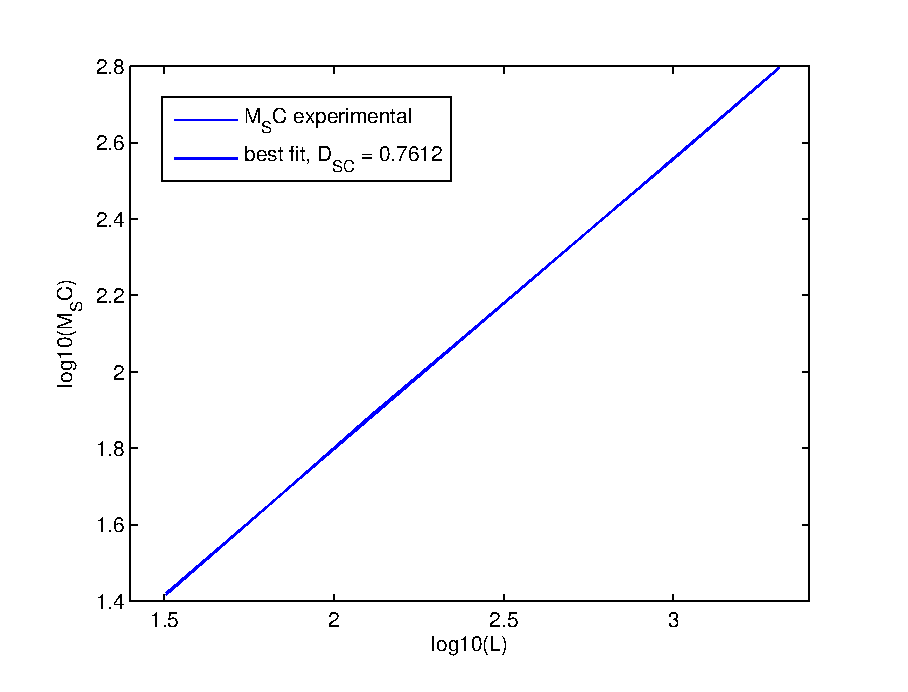
\includegraphics[width=13cm]{dsc.eps}
	%\label{fig:subfig51}


\caption[Optional caption for list of figures]{The figure shows $M_SC$ as a function of $L$.}
\label{fig:11}
\end{figure}

We can also investigate the behaviour of $P_{SC} = M_{SC}/L^d$ as a function of $p-p_c$. This investigation is summarized in figure \ref{fig:12}

\begin{figure}[ht]
\subfigure[$P_{SC}$ for various $L$]{
	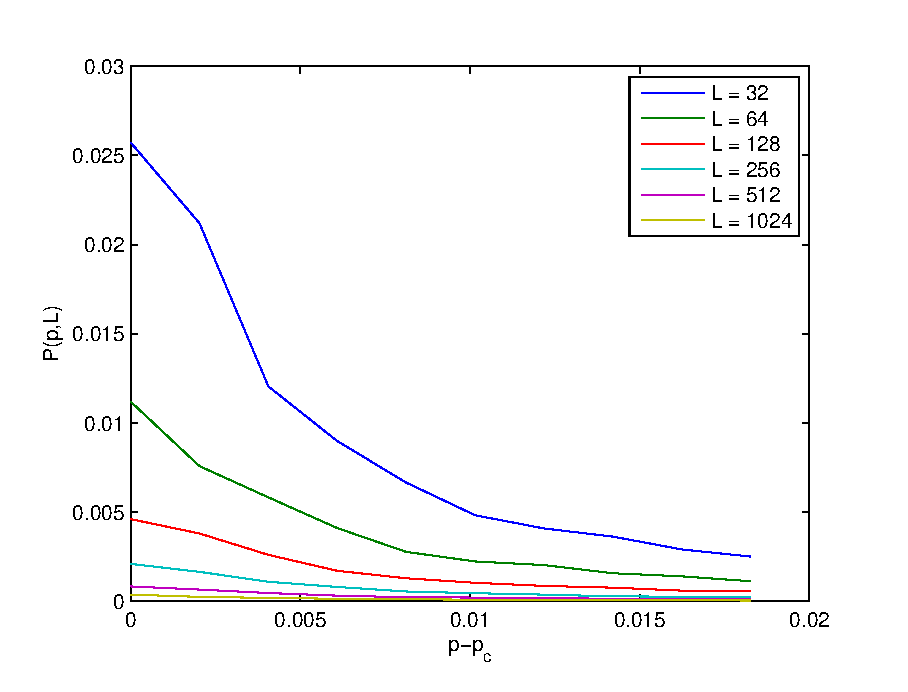
\includegraphics[width=7cm]{P_SC.eps}
	\label{fig:subfig121}
}
\subfigure[Data collapse of $P_{SC}$]{
	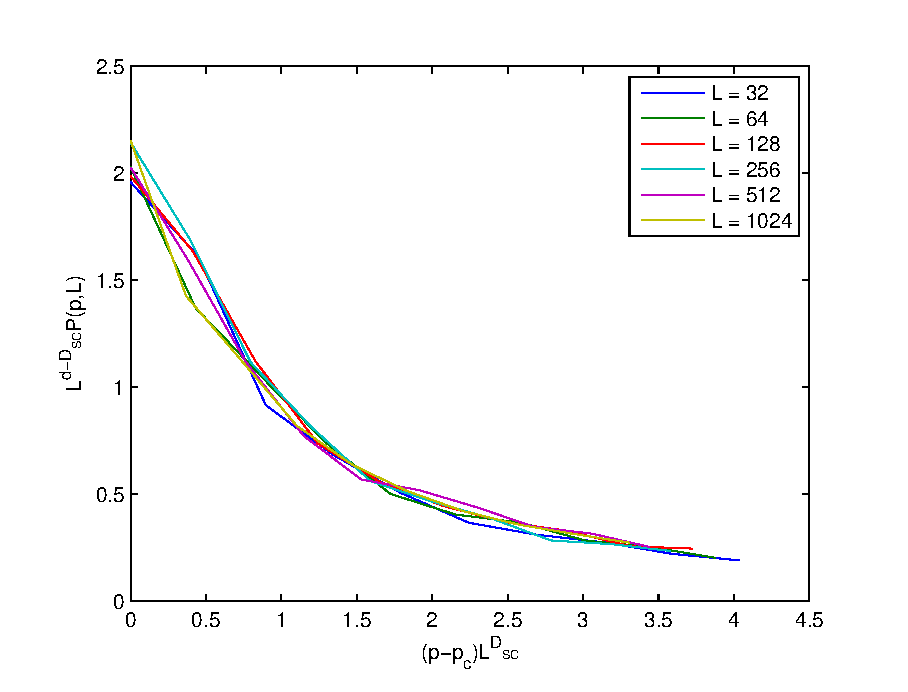
\includegraphics[width=7cm]{P_SC_datacoll.eps}
	\label{fig:subfig122}
}
\caption[Optional caption for list of figures]{The figures show $p_{\Pi=x}$ as a function of $L$.}
\label{fig:12}
\end{figure}

\clearpage

\section{Flow on fractals}
In this section we study flow on a spanning percolating cluster. A percolating cluster can be broken down to the component shown in fig \ref{fig:tef}. I.e. backbone, dangling ends and singly connected bonds. For flow problems, note that all the fluid will travel through the singly connected bonds, while none will travel through the dangling ends.


\begin{figure}[ht]
\centering

	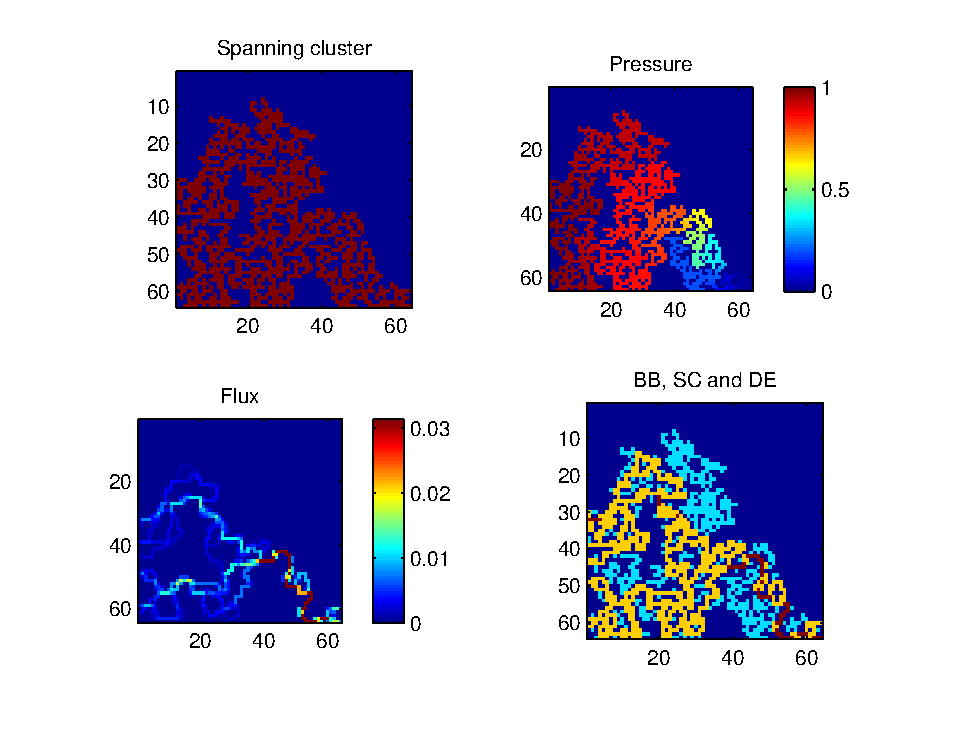
\includegraphics[width=13cm]{testexflow.eps}
	%\label{fig:subfig51}


\caption[Optional caption for list of figures]{The figure shows properties of flow through a percolating cluster.}
\label{fig:tef}
\end{figure}

 We can investigate the dimensionality of the different subsets of the percolating cluster. This is shown in figure \ref{fig:massd}. Note that surprisingly, $D_{DE} \approx 2.14 > 2$! This will probably not hold for very large systems, as the dangling ends would then at some point usurp the whole system. 
 
  \begin{figure}[ht]
\centering

	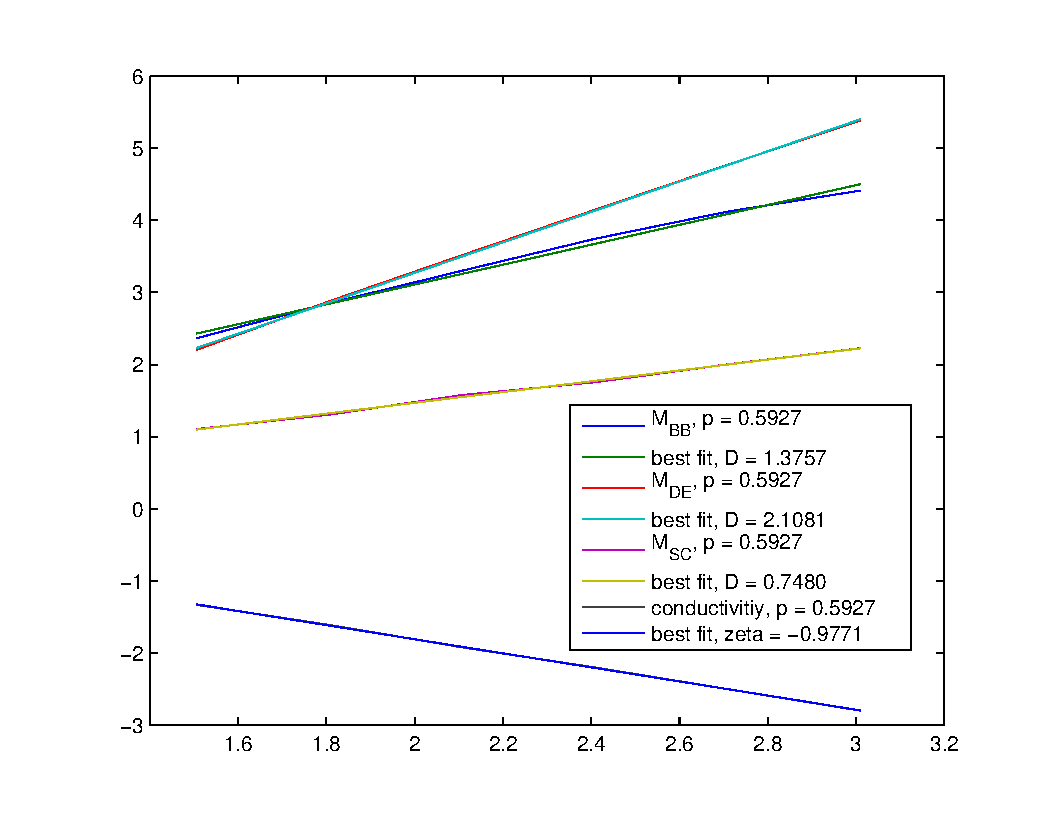
\includegraphics[width=13cm]{massdims.eps}
	%\label{fig:subfig51}


\caption[Optional caption for list of figures]{The figure shows the dimensional behaviour of different properties at $p=p_c$.}
\label{fig:massd}
\end{figure}
 
 The we note that the the scaling exponent $\tilde{\zeta}_R \approx 0.97$. We can also measure the conductivity as a function of $p-p_c$. From the scaling theory, $\sigma \propto (p-p_c)^\mu$, where $\mu$ is the conductivity. From figure \ref{fig:mp}, we see that for large systems, $\mu \approx 1.28$.
 

 \begin{figure}[ht]
\centering

	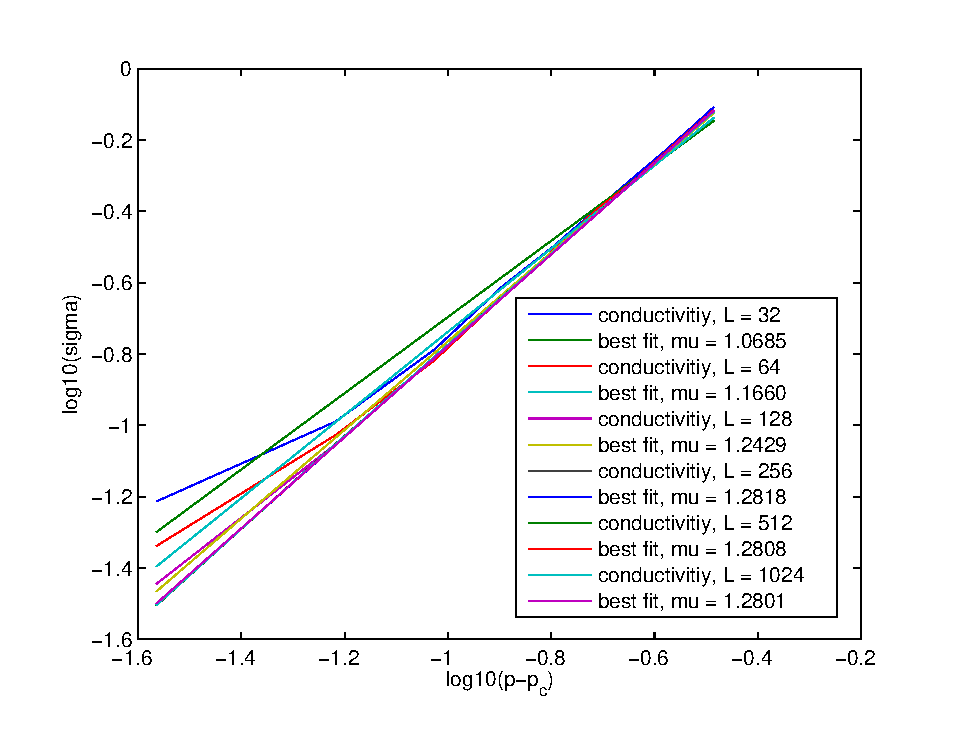
\includegraphics[width=13cm]{muofp.eps}
	%\label{fig:subfig51}


\caption[Optional caption for list of figures]{The figure shows the conductivity as a function of $p-p_c$ for various $L$.}
\label{fig:mp}
\end{figure}



\clearpage
\section{Random walks on a percolating cluster}
In this last section we will experiment with letting a random walker move freely around on a percolating cluster, as illustrated in figure \ref{fig:13}. We can find the distance $\langle R^2 \rangle$ as a function of the number of steps $N$ for $p>p_c$. The result of this is shown in figure \ref{fig:14}. We see that $\langle R^2 \rangle $ approaches 1 as $p \rightarrow 1$, as is expected from normal diffusion theory. 

\begin{figure}[ht]
\centering

	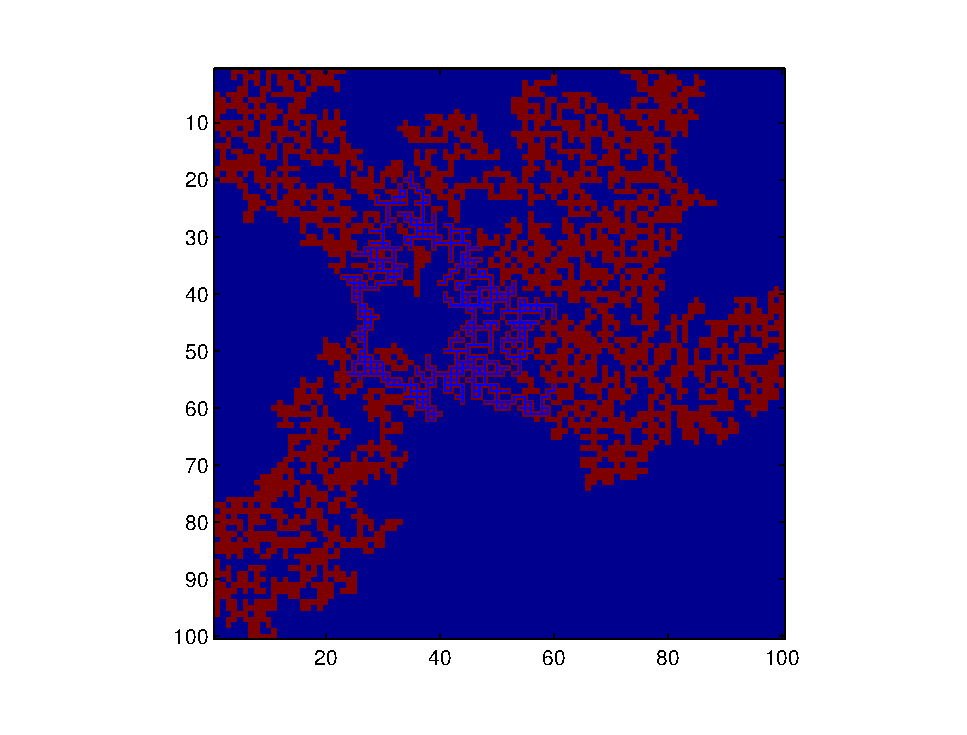
\includegraphics[width=13cm]{percex.eps}
	%\label{fig:subfig51}


\caption[Optional caption for list of figures]{The figure shows an example of a random walk on a percolating cluster.}
\label{fig:13}
\end{figure}

\begin{figure}[ht]
\centering

	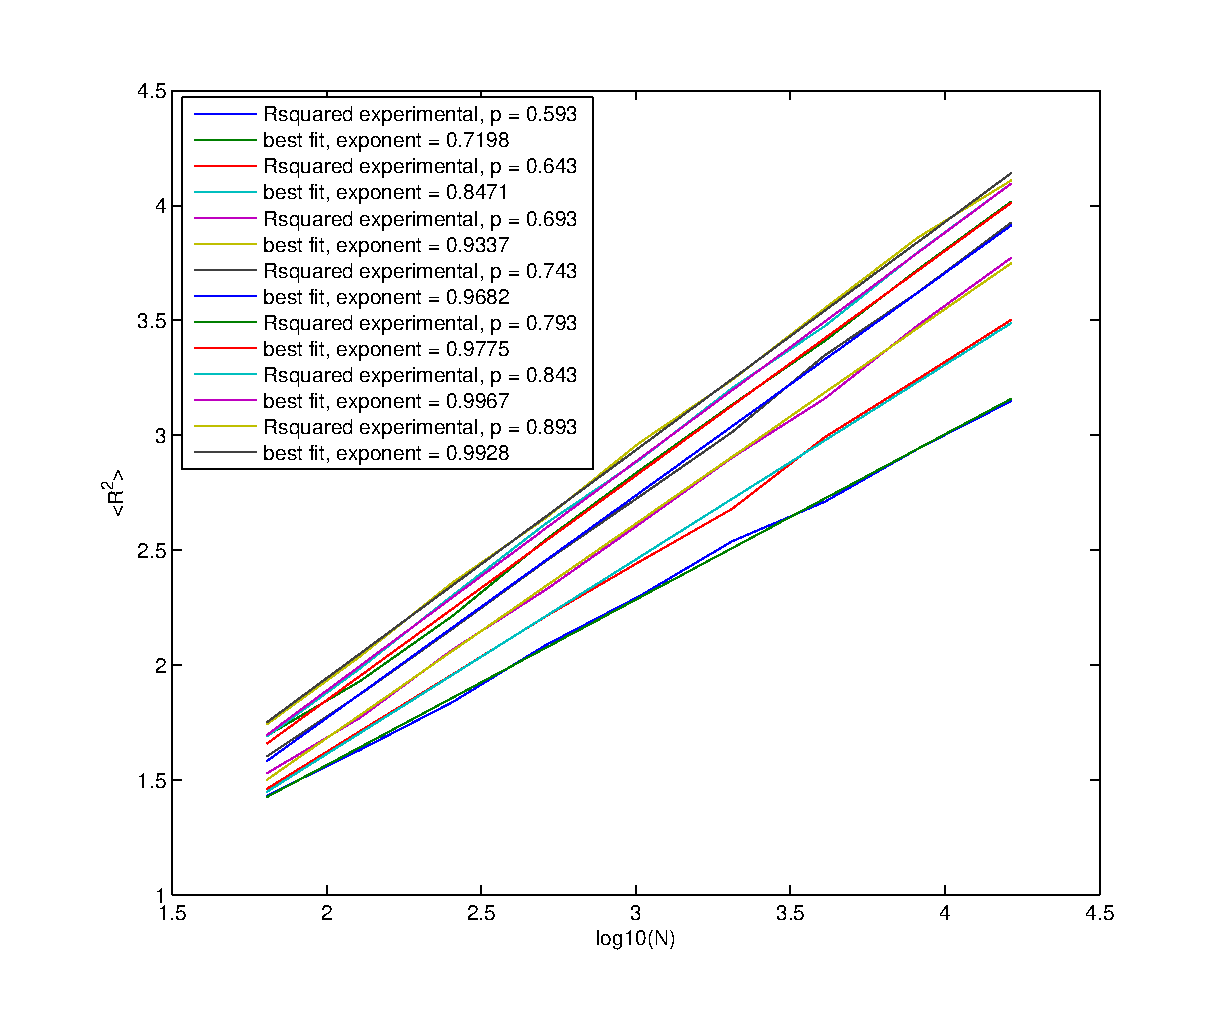
\includegraphics[width=13cm]{rofn.eps}
	%\label{fig:subfig51}


\caption[Optional caption for list of figures]{The figure shows $\langle R^2 \rangle$ as a function of $N$ for various $p$.}
\label{fig:14}
\end{figure}

Diffusion theory tells us that in general, 

\begin{equation}
 \langle R^2 \rangle \propto t^{2/d_w}
\end{equation}
where $d_w$ is the dimension of the random walker, which can be shown to be 
\begin{equation}
 d_w = 2 + {\mu \over \nu - {\beta \over 2}}.
\end{equation}
where $\mu$ is the conductivity of the cluster. We note that for $p = p_c$, $d_w \approx 2.76$.

%The results from figure \ref{fig:14} can be used to find $\mu$, as illustrated in figure \ref{fig:15}. We find that $\mu \approx ...$.

The rest of this exercise falls appart...  It is not possible to get good data for $\langle R^2 \rangle$ for $p>p_c$

%Finally, the dimension $d_w$ of the walk can be found from $\langle R^2 \rangle \propto N^{2/d_w}$, which gives us that $d_w \approx ...$

\end{document}